\chapter{Configuration}\label{cha:configuration}
XCSoar is a highly configurable glide computer and can be customised
to suit a wide variety of preferences and user requirements.  This
chapter describes the configuration settings and options.

\section{Scope of configuration}

There are several ways XCSoar can be customised:
\begin{itemize}

\item Modifying configuration settings.  This is the sort of configuration
 most likely to be performed by users; and this is given the greatest attention in this document.
\item Changing the language, or even just to change the wording
  of text in the user interface.
\item Changing the button assignments and button menus.  This allows 
the content and structure of the button menu to be changed. 
\item Changing or adding actions performed when glide computer events
 take place.
\item Defining how long status messages appear and sounds to be played
 when those messages occur.
\end{itemize}
Describing all of these in a detail level like a reference manual would 
do is beyond the scope of this document. The user is referred to browse 
through the XCSoar Wiki for more details. 
\url{http://www.xcsoar.org/trac/wiki}

\section{Modifying settings}

There are a large set of configuration settings that may be customised
from the Settings dialogue accessible from the menu under
\begin{quote}
\bmenu{Config}\blink\bmenu{Config}\blink\bmenu{Setup system}
\end{quote}

You are strongly discouraged from changing these settings during
flight.  \warning  All changes to the settings should be performed on the ground
so that their desired effect on the programs behaviour can be
verified.

The settings dialogue contains several pages.  Once changes have been made,
click the Close button on the screen or PWR/ESC on Altair to close the dialogue
and return the program back to normal map mode.

\tip Once you are happy with your configuration settings, save the
profile file and make a backup so that you can later restore the
settings if your PDA's memory is accidentally erased.

See Chapter~\ref{cha:data-files} for a description of the data formats
of files referred to in the settings.  Where no file is to be used,
the field can be left blank.  File name fields in forms show files
that match a file extension filter.  This makes it much easier to find
and select the correct file.

The main configuration dialogue (Setup System) can be run in Basic or
Expert user level, via a selectable field on the left of the dialogue.
When in Basic mode, many of the less commonly used and advanced
configuration settings are hidden.  In the descriptions below,
all of the parameters marked with an asterisk are only visible in
expert user level.

Basic user level:
\begin{center}
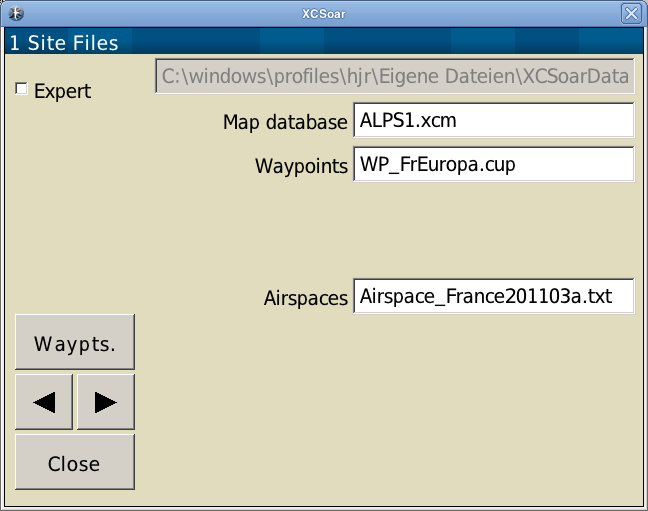
\includegraphics[angle=0,width=0.8\linewidth,keepaspectratio='true']{figures/config-basic.png}
\end{center}

Expert user level:
\begin{center}
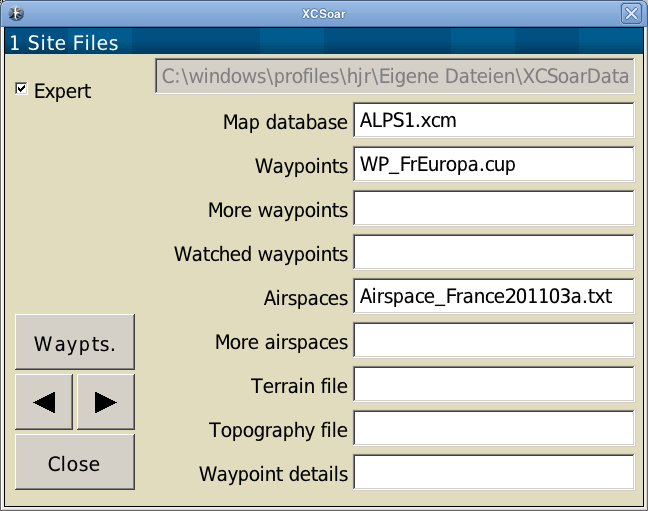
\includegraphics[angle=0,width=0.8\linewidth,keepaspectratio='true']{figures/config-expert.png}
\end{center}

%\subsection*{Fail-safe}

%If the XCSoar software crashes due to an unrecoverable error while
%loading a file, the file will be removed from the configuration
%settings in order to prevent the crash reoccurring.  Therefore, if an
%error was found in a file, the user must re-enter that file in the
%configuration settings after remedying the situation.


%%%%%%%%%%%%%%%%%%
\clearpage
\section{Site files}
The dialogue specifies most of the important files that must be
configured when flying at a new site.

\begin{center}
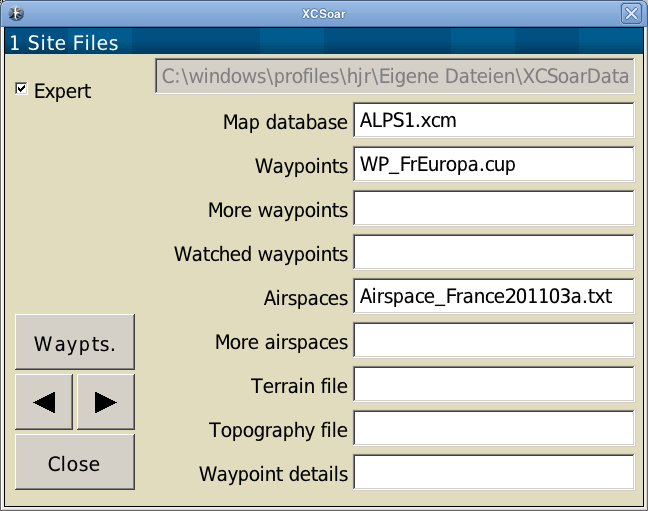
\includegraphics[angle=0,width=0.8\linewidth,keepaspectratio='true']{figures/config-site.png}
\end{center}

\begin{description}
\item[XCSoar data path]  The location for all of your XCSoar data on your hard drive, 
  SD card, or the PDA's static memory.
\item[Map Database]  The name of the map file (XCM) containing digital elevation
  terrain data, topography, and optionally waypoints, airspace etc. A good
  prepared database file covers all the needs for this page.
\item[Waypoints]  Primary waypoints file.  If left blank, waypoints are loaded
from the map file (if available).
\item[More waypoints*]  Secondary waypoints file.  This may be used to add waypoints for a competition.
\item[Watched waypoints*]  Waypoint file containing special waypoints for which additional computations 
  like calculation of arrival height in map display always takes place. Useful for waypoints 
  like known reliable thermal sources (e.g. powerplants) or mountain passes.
\item[Airspaces]  The file name of the primary airspace file.  If left blank,
airspaces are loaded from the map file (if available).
\item[More airspaces*]  The file name of the secondary airspace file.
\item[Terrain file*]  The name of the file containing digital elevation
  terrain data.  Typically left blank, because terrain is loaded from the map
  file.
\item[Topography file*]  Specifies the file defining the topographical features.
The topography file defines the map topography in terms of points, lines
and areas with optional labels.  Typically left blank, because topography is
loaded from the map file.
\item[Waypoint details*]  The airfields file may contain extracts from Enroute Supplements or
other contributed information about individual airfields.
\end{description}

Airspace files define Special Use Airspace.  Up to two files may be
specified, the first for the main SUA file, and the second is intended
for use with NOTAM airspace, and is referred to as the additional
airspace file.

The XCM map database concept is the recommended way to setup a site to fly.
The old method (XCSoar v5.x) requires each to be separate files and to be
specified separately (as the ``Terrain file'' and ``Topography file'' respectively).  

When XCM map files are used, however, then these files contain terrain, topography
and optionally waypoints.  In this case, the ``Terrain file'', ``Topography file'' and 
``Primary waypoint file'' may be left blank and the system will load those items
from the map file. However, if a map file is used, the use can still specify the other
files and they will be used instead of the data in the map file.

See Section~\ref{sec:map} for more details on map files.


%%%%%%%%%%%%%%%%%%
\clearpage
\section{Map projection}\label{sec:map-projection}

This page let you specify the favoured map orientation and projection.

\begin{center}
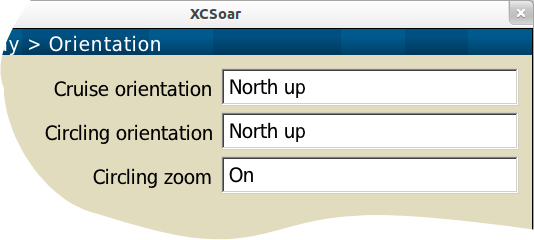
\includegraphics[angle=0,width=0.8\linewidth,keepaspectratio='true']{figures/config-map_projection.png}
\end{center}

\begin{description}
\item[Cruise/Circling orientation]  \label{conf:orientation} This determines how
  the screen is rotated with the glider, depending on it's current display mode. \\
  {\bf Track up}: The moving map display will be rotated so the glider's track
  is oriented up. The north arrow symbol points to true north. The glider symbol 
  may be shown rotated according to the computed heading of the glider taking 
  wind into account. \\
  {\bf North up}: The moving map display will always be orientated true north to
  south and the glider icon will be rotated to show its course (corrected for
  wind). \\
  {\bf Target up}: The moving map display will be rotated so the current target
  direction is oriented up.
\item[Circling zoom]  \label{conf:circlingzoom} This determines whether separate
  zoom levels will be maintained for circling and cruise modes.  If enabled, then the 
  map will zoom in automatically when entering circling mode and zoom out
  automatically when leaving circling mode.
\item[Map shift reference]  The direction according to the map will be displaced 
  in order to present a meaningful map section. \\
  {\bf None}: Disable any adjustment. \\
  {\bf Track}: Use a recent average of the ground track as basis. \\
  {\bf Target}: Use the current target waypoint as basis.
\item[Glider position offset]  \label{conf:gliderposition} Defines the location of the 
  glider drawn on the screen in percent from the screen edge.
\item[Max. auto zoom distance]  The upper limit for auto zoom distance.
\end{description}


%%%%%%%%%%%%%%%%%%
\clearpage
\section{Map elements}\label{sec:map-elements}

This page provides options relating to screen elements overlayed to the map display.

\begin{center}
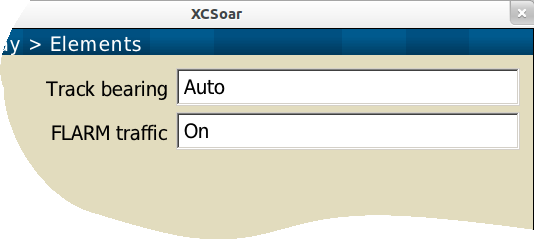
\includegraphics[angle=0,width=0.8\linewidth,keepaspectratio='true']{figures/config-map_elements.png}
\end{center}

\begin{description}
\item[Track bearing]  Display the ground track (ground track projection) on the map.
  The setting "Auto" displays the ground track only if there is a significant 
  difference to plane heading.
\item[FLARM traffic]  \label{conf:flarm-on-map} This enables the display of FLARM 
  traffic on the map.
\item[Trail length*] \label{conf:snailtrail} Determines whether and how long a
  snail trail is drawn behind the glider. \\
  {\bf Off}: No trail is drawn. \\
  {\bf Long}: A long trail is drawn (approx 60 minutes). \\
  {\bf Short}: A short trail is drawn (approx 10 minutes). \\
  {\bf Full}: A trail for the entire flight is drawn.
\item[Trail drift*] \label{conf:traildrift} Determines whether the
  snail trail is drifted with the wind when displayed in circling mode.  Switched Off,
  the snail trail stays uncompensated for wind draft.
\item[Trail type*] \label{conf:snailtype} Sets the type of the snail trail display. \\
  {\bf Vario \#1}: Within lift areas lines get displayed green and
  thicker, while sinking lines are shown red and thin.  Zero lift
  is presented as a grey line. \\
  {\bf Vario \#2}: The climb colour for this scheme is orange to red, sinking is
  displayed as light blue to dark blue. Zero lift is presented as a yellow line. \\
  {\bf Altitude}: The colour scheme corresponds to the height.
\item[Trail scaled*] \label{conf:trailscaled} If activates, the snail trail width 
  is scaled according to the vario signal.
\item[Detour cost markers*]  If enabled this displays in cruise flight some
  figures projected in front of the nose of the glider icon.  This is the
  additional distance in percent if you fly up the position of the figure and
  after that again straight towards the target, compared to the straight distance
  to target.
\item[Aircraft symbol*]  Sets the symbol used for the aircraft. \\
  {\bf Simple}: Simplified line graphics, a black glider shape with white contours. \\
  {\bf Simple (large)}: Enlarged simple graphics for better visibility on a small display. \\
  {\bf Detailed}: Rendered aircraft graphics.
\item[Wind arrow*]  Determines the way the wind arrow is drawn on the map. \\
  {\bf Arrow head}: Draws an arrow head only. \\
  {\bf Full arrow}: Draws an arrow head with a dashed arrow line.
\end{description}


%%%%%%%%%%%%%%%%%%
\clearpage
\section{Waypoint display}\label{sec:waypoint-display}

This page provides options relating to the map display.

\begin{center}
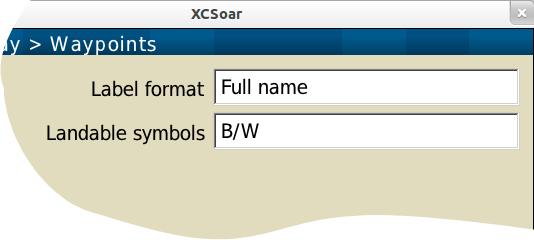
\includegraphics[angle=0,width=0.8\linewidth,keepaspectratio='true']{figures/config-map_waypoint.png}
\end{center}

\begin{description}
\item[Label format]  This setting \label{conf:labels} determines the label format 
  displayed with each waypoint. There are four different format options.
  {\bf Full name}: The full name of each waypoint is displayed. \\
  {\bf First word of name}: Only the first word (up to the first space) of the 
  waypoint name is displayed. \\
  {\bf First 3}: The first 3 letters of the waypoint name are displayed. \\
  {\bf First 5}: The first 5 letters of the waypoint name are displayed. \\
  {\bf None}: No name is displayed with the waypoint.
\item[Arrival height*]  This enables the arrival height info shown additionally 
  for landables. \\
  {\bf None}: No arrival height is displayed. \\
  {\bf Straight glide}: Straight glide arrival height (no terrain is considered). \\
  {\bf Terrain avoidance glide}: Arrival height considering terrain avoidance. \\
  {\bf Straight \& terrain glide}: Both arrival heights are displayed.
\item[Label style*]  Labels for lanbables can be shown on a rounded rectangle with 
  white background, or with outlined letters.
\item[Waypoint label visibility*]  \label{conf:labelvisibility} Controls which waypoints 
  are displayed with names and arrival altitudes on the map: \\
  {\bf All}: All waypoint labels will be displayed. \\
  {\bf Task waypoints and landables}: All waypoints part of a task and all landables 
  will be displayed. \\
  {\bf Task waypoints}: All waypoints part of a task will be displayed. \\
  {\bf None}:  No waypoint labels will be displayed.
\item[Landable symbols]  \label{conf:waypointicons} Three styles are available:
  Purple circles (WinPilot style), a high contrast style with icons,
  and icons with a traffic light colour scheme. See Section~\ref{sec:waypoint-schemes} for details.
\item[Detailed landables*]  Enabling details on landables displays instead of fixed icons 
  variable information like runway length and heading.
\item[Landable size]  A percentage to select the size landables are displayed on the map.
\item[Scale runway length]  Enabling this option will display for detailed landables 
  additionally a scaled runway length based on real length.
\end{description}


%%%%%%%%%%%%%%%%%%
\clearpage
\section{Terrain display}\label{sec:terrain-display}

This page sets how terrain and topography is drawn on the map window.

\begin{center}
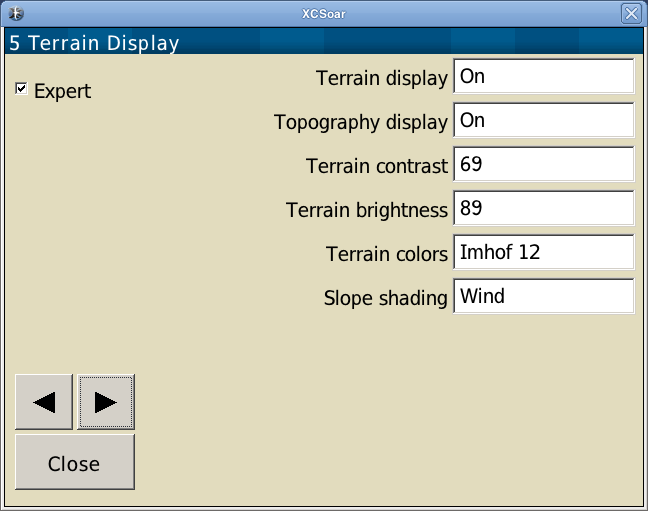
\includegraphics[angle=0,width=0.8\linewidth,keepaspectratio='true']{figures/config-terrain.png}
\end{center}

\begin{description}
\item[Terrain display]  Draws digital elevation terrain on the map.
\item[Topography display]  Draws topographical features (roads, rivers, lakes etc.) on
 the map.
\item[Terrain contrast*]  Defines the amount of Phong shading in the terrain rendering. 
 Use large values to emphasise terrain slope, smaller values if flying in steep mountains.
\item[Terrain brightness*]  Defines the brightness (whiteness) of the terrain rendering. 
 This controls the average illumination of the terrain.
\item[Terrain colours]  Defines the colour ramp used in terrain rendering.  Various 
 schemes are available, which works best for you will depend on how mountainous your region is.
\item[Slope shading*]  \label{conf:shading} The terrain can be shaded among slopes 
 to indicate either wind direction, sun position or a fixed shading from north-east. 
 Slopes faced to the wind (or sun) get displayed brighter and the averted slopes get darker.
\end{description}


\begin{maxipage}
The available terrain colour schemes are illustrated in the table below.

\begin{longtable}{c c c c}
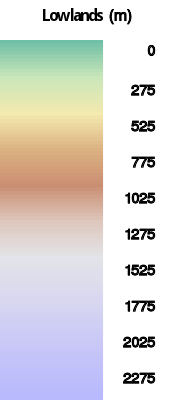
\includegraphics[angle=0,width=3.5cm,keepaspectratio='true']{figures/ramp-terrain-flatlands.png}&
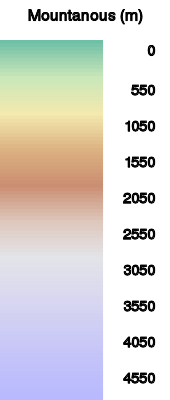
\includegraphics[angle=0,width=3.5cm,keepaspectratio='true']{figures/ramp-terrain-mountanous.png}&
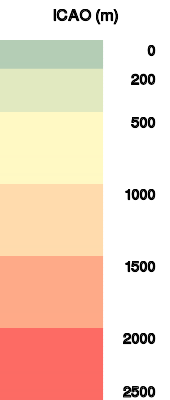
\includegraphics[angle=0,width=3.5cm,keepaspectratio='true']{figures/ramp-terrain-icao.png}&
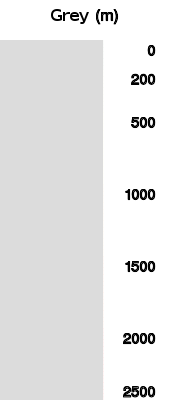
\includegraphics[angle=0,width=3.5cm,keepaspectratio='true']{figures/ramp-terrain-grey.png}
\\

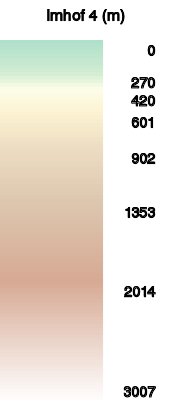
\includegraphics[angle=0,width=3.5cm,keepaspectratio='true']{figures/ramp-terrain-imhof4.png}&
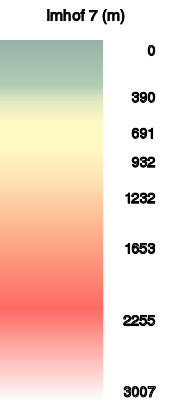
\includegraphics[angle=0,width=3.5cm,keepaspectratio='true']{figures/ramp-terrain-imhof7.png}&
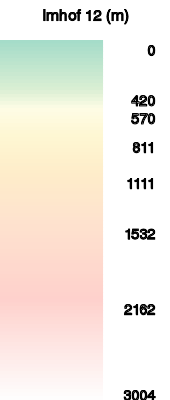
\includegraphics[angle=0,width=3.5cm,keepaspectratio='true']{figures/ramp-terrain-imhof12.png}&
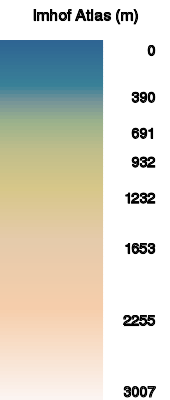
\includegraphics[angle=0,width=3.5cm,keepaspectratio='true']{figures/ramp-terrain-imhofatlas.png}
\\
\end{longtable}
\end{maxipage}


%%%%%%%%%%%%%%%%%%
\clearpage
\section{FLARM and other gauges} \label{sec:vario-gauge}

\begin{center}
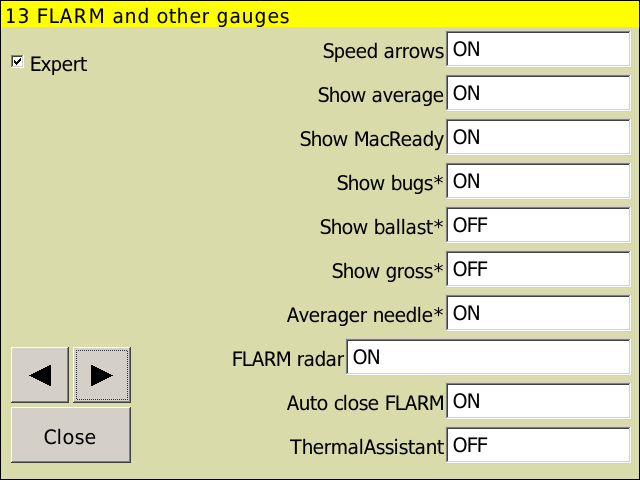
\includegraphics[angle=0,width=0.8\linewidth,keepaspectratio='true']{figures/config-othergauges.png}
\end{center}

\begin{description}
\item[FLARM radar]  \label{conf:flarmdisplay} This enables the display of the FLARM 
  radar gauge. The track bearing of the target relative to the track bearing of the 
  aircraft is displayed as an arrow head, and a triangle pointing up or down shows 
  the relative altitude of the target relative to you.
\item[Auto close FLARM*]  This will close the FLARM radar view when all FLARM traffic has gone.
\item[ThermalAssistant] \label{conf:thermalassistant} Enables the display of the
  thermal assistant gauge.

\item[Speed arrows*]  \label{conf:variogauge} Whether to show speed command 
  arrows on the vario gauge.
  When shown, in cruise mode, arrows point up to command slow down; arrows point down 
  to command speed up.
\item[Show average*]  Whether to show the average climb rate.  In cruise mode, this 
  switches to showing the average net airmass rate.
\item[Show MacCready*]  Whether to show the MacCready setting.
\item[Show bugs*]  Whether to show the bugs percentage.
\item[Show ballast*]  Whether to show the ballast percentage.
\item[Show gross*]  Whether to show the gross vario value.
\item[Averager needle*]  If true, the vario gauge will display a hollow averager
  needle. During cruise, this needle displays the average net value. During circling, 
  this needle displays the average gross value.
\end{description}

In all FLARM environment, the colour of the target indicates the threat level.


%%%%%%%%%%%%%%%%%%
\clearpage
\section{Glide computer}\label{sec:final-glide}

This page allows glide computer algorithms to be configured.

\begin{center}
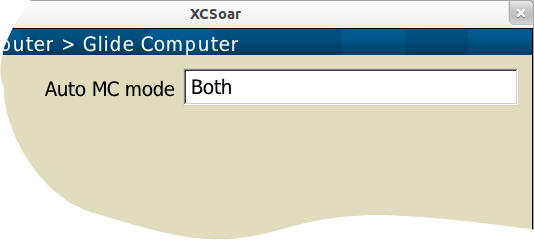
\includegraphics[angle=0,width=0.8\linewidth,keepaspectratio='true']{figures/config-glidecomputer.png}
\end{center}

\begin{description}
\item[Auto wind]  \label{conf:autowind} This allows switching on or off the
  automatic wind algorithm. \\
  {\bf Manual}: When the algorithm is switched off, the pilot is responsible for
  setting the wind estimate. \\
  {\bf Circling}: Circling mode requires only a GPS source. \\
  {\bf ZigZag}: ZigZag requires an intelligent vario with airspeed output. \\
  {\bf Both}:  Uses Circling and ZigZag.
\item[External wind]  If enabled, the wind vector received from external
  devices overrides XCSoar's internal wind calculation.
\item[Auto MC mode]  This option defines which auto MacCready algorithm is used.
  For more details see Section~\ref{sec:auto-maccready}. \\
  {\bf Final glide}: Final glide adjusts MC for fastest arrival. \\
  {\bf Trending average climb}: Sets MC to the trending average climb rate based 
  on all climbs. \\
  {\bf Both}: Uses trending average during task, then fastest arrival when in final 
  glide mode.
\item[Block speed to fly*]  If enabled, the command speed in cruise
  is set to the MacCready speed to fly in no vertical air-mass movement.
  If disabled, the command speed in cruise is set to the dolphin speed to fly,
  equivalent to the MacCready speed with vertical air-mass movement.
\item[Nav by baro altitude*]  When enabled and if connected to a barometric
  altimeter, barometric altitude is used for all navigation functions. Otherwise
  GPS altitude is used.
\item[Flap forces cruise*]
  When this option is enabled, causes the flap switches in Vega to
  force cruise mode when the flap is not positive. This means that
  when departing a thermal, switching to neutral or negative flap will
  immediately switch XCSoar's mode to cruise mode.
  Similarly, for Borgelt B50 systems, the speed command switch forces
  XCSoar's climb or cruise mode.
\item[L/D Average period*]  Average efficiency is always calculated in real-time. 
  Here you can decide on how many seconds of flight this calculation must be done. 
  The real distance covered second by second in this period is divided by the final 
  difference of altitude.  So if for example you go and return back to the same point 
  after 2 minutes, and you have set 2 minutes as period, average LD will consider the 
  total distance covered in those two minutes , and not the distance between your 
  position 2 minutes before and your current position, that in this case could be 
  almost zero! Normally for gliders a good value is 90-120 seconds, and for paragliders 
  15 seconds. Lower values will give as a result pretty much the same as LD Instant, 
  while higher values will look like LD Cruise. Other commercial instruments and 
  software use 2 minutes.
\end{description}


%%%%%%%%%%%%%%%%%%
\clearpage
\section{Safety factors}

This page allows the safety heights and behaviour in abort mode to be defined.

\begin{center}
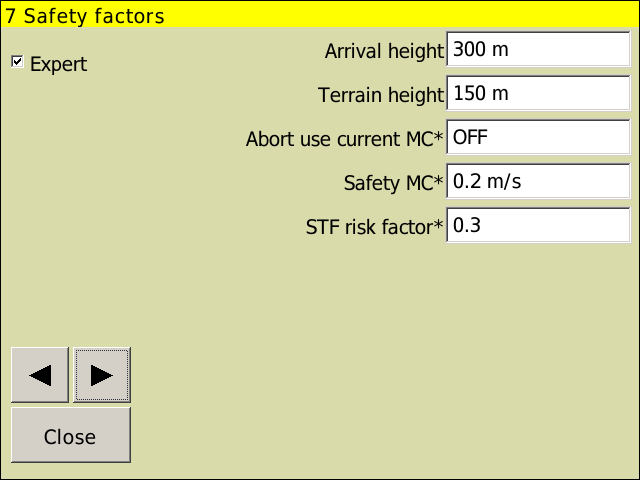
\includegraphics[angle=0,width=0.8\linewidth,keepaspectratio='true']{figures/config-safety.png}
\end{center}

\begin{description}
\item[Arrival height]  The height above terrain that the glider
  should arrive at for a safe landing.
\item[Terrain height]  \label{conf:safetyterrain} The height above terrain that the glider must
  clear during final glide.
\item[Alternates mode]  \label{conf:alternatesmode} Determines sorting of alternates 
  in the alternates dialogue and in abort mode. \\
  {\bf Simple}: The alternates will only   be sorted by waypoint type 
  (airport/outlanding field) and arrival height. \\
  {\bf Task}: The sorting will also take the current task direction into account. \\
  {\bf Home}: The sorting will try to find landing options in the current direction 
  to the configured home waypoint.
\item[Safety MC*]  The MacCready setting used for reach calculations, task abort, alternates and
  for determining arrival altitude at airfields. 
\item[STF risk factor*] 
  The STF risk factor reduces the MacCready setting used to calculate
  speed to fly as the glider gets low, in order to compensate for
  risk.  Set to 0.0 for no compensation, 1.0 scales MC linearly with
  height.  See Section~\ref{sec:speed-fly-with} for more details.
\end{description}
See Section~\ref{sec:safety-heights} for more details on the meanings
of the safety heights.


%%%%%%%%%%%%%%%%%%
\clearpage
\section{Route}

This page allows control over glide reach calculations and route
optimisations.

\begin{center}
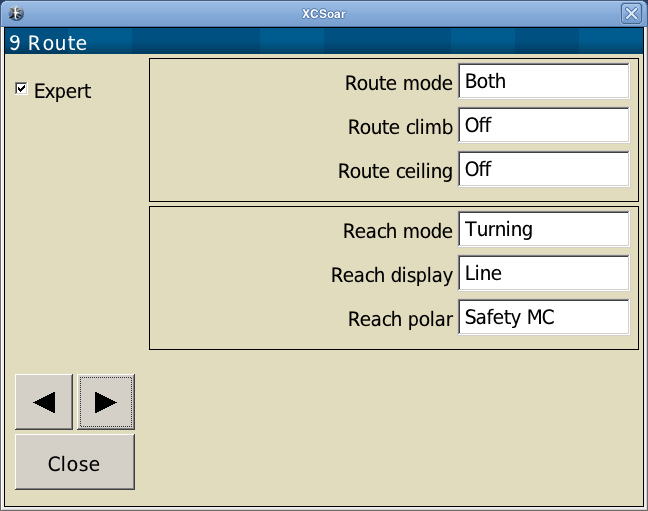
\includegraphics[angle=0,width=0.8\linewidth,keepaspectratio='true']{figures/config-route.png}
\end{center}

\begin{description}
\item[Route mode]  \label{conf:routemode} This controls which types
  of obstacles are used in route planning.
\item[Route climb*]  \label{conf:routeclimb} When enabled and Mc is positive, route 
  planning allows climbs between the aircraft location and destination.
\item[Route ceiling*]  \label{conf:routeceiling} When enabled, route planning climbs 
  are limited to ceiling defined by greater of current aircraft altitude plus 
  500 m and the thermal ceiling.  If disabled, climbs are unlimited.
\\
\item[Reach mode]  \label{conf:turningreach} How calculations are performed of 
  the reach of the glider with respect to terrain. \\
  {\bf Off}: Reach calculations disabled. \\
  {\bf Straight}: The reach is from straight line paths from the glider. \\
  {\bf Turning}: The reach is calculated allowing turns around terrain obstacles.
\item[Reach display]  \label{conf:gliderange} This determines whether the
glide reach is drawn as a line resp.\ a shade on the map area.
\item[Reach polar*]  \label{conf:reachpolar} This determines the glide performance 
  used in reach, landable arrival, abort and alternate calculations. \\
  {\bf Task}: Uses task glide polar; \\
  {\bf Safety MC}: Uses safety MacCready value.
\end{description}


%%%%%%%%%%%%%%%%%%
\clearpage
\section{Polar}

This page allows the glide polar to be defined. For a large variety of glider types 
XCSoar provides a predefined glide polar, they could be modified if needed, or 
you can load your own polar from a file. 
The file format is based on the WinPilot polar file format (see section~\ref{sec:glide-polar}).

\begin{center}
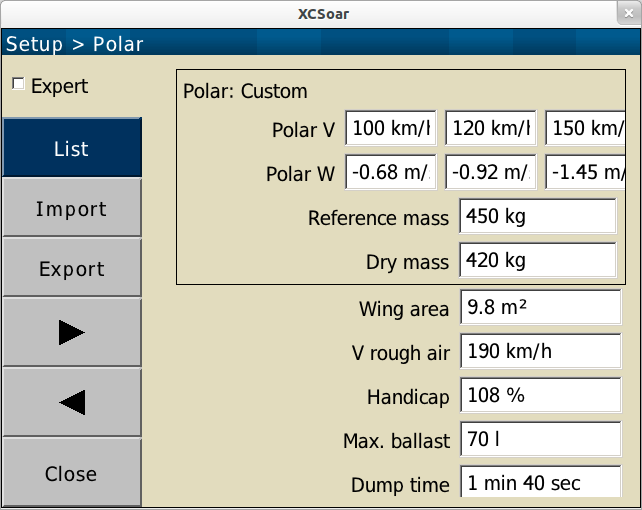
\includegraphics[angle=0,width=0.8\linewidth,keepaspectratio='true']{figures/config-polar.png}
\end{center}

\label{conf:polar} To configure the glide computer to the performance of a glider 
type start with the selection of a type from the \button{List}. 
Choose \button{Import} when you want to load an external polar file.
Customize the three V/W points defining the parable curve and the reference 
weight to your needs. 
\tip Be aware that namely those four items are of crucial importance 
for every glide performance relevant computation of XCSoar.   
\button{Export} your efforts to a file is always a good idea.

\begin{description}
\item[Polar V/W*]  Pair of corresponding horizontal and vertical speed of the glider. 
  A good choice for the point triplet is one at the top most area of the polar, the second at a 
  still very curved area and the third far out where the curvature seems to disappear.
\item[Ref. mass*]  Reference weight at which the given polar is valid.
\item[Max. ballast]  Optional the amount of water ballast XCSoar refers to as 100\% ballast.
  Set to zero if it does not apply.
\item[Wing area*]  Optional specification of the wing area of the glider type.
\item[V rough air*] Optional the maximum manoeuvring speed can 
  be entered on this page to prevent the glide computer from commanding 
  unrealistic cruise speeds.
\item[Handicap*]  The handicap factor used for the OnLine Contest scoring.
\item[Dump time*]  The time in seconds needed for dumping full ballast.
\end{description}


%%%%%%%%%%%%%%%%%%
\clearpage
\section{Airspace}

This page is used to determine how the airspace information is
displayed and how warnings are issued.

\begin{center}
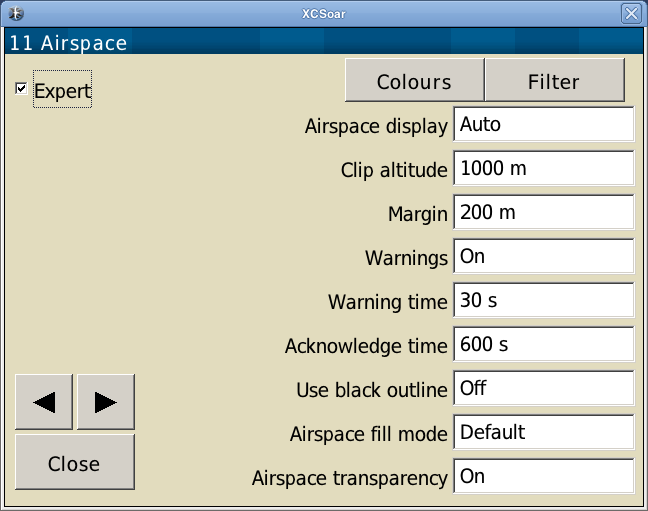
\includegraphics[angle=0,width=0.8\linewidth,keepaspectratio='true']{figures/config-airspace.png}
\end{center}

\begin{description}
\item[Airspace display]  Controls how airspace display and warnings are filtered 
  based on altitude.  The airspace filter dialogue also allows filtering
  of display and warnings independently for each airspace class. \\
  {\bf All on}: All the airspace information is displayed at the same time. \\
  {\bf Clip}: Only airspace below a user determined altitude is shown. \\
  {\bf Auto}: Only airspace at the current altitude plus or minus a user definable margin is shown. \\
  {\bf All below}:  Only airspace below the glider is shown.
\item[Clip altitude] For clip mode, this is the altitude below which airspace is displayed.
\item[Margin]  For auto airspace mode, this is the height above/below which airspace is included.
\item[Warnings]  Determines whether warnings are enabled or disabled.
\item[Warning time*]  This is the time before an incursion is estimated at
  which the system will warn the pilot.
\item[Acknowledge time*]  This is the time period in which an acknowledged airspace 
  warning will not be repeated.
\item[Use black outline*]  Draws a black outline around each airspace.
\item[Airspace fill mode*]  Specifies the mode for filling the airspace area. \\
  {\bf Fill all}:  Transparently fills the airspace colour over the whole area. \\
  {\bf Fill padding}: Draws a solid outline with a half transparent border around the airspace. \\
  {\bf Default}:  This selects the best performing option for your hardware. In fact 
  it favours "fill padding" except for PPC 2000 system.
\item[Airspace transparency*]  If enabled, then airspaces are filled transparently.
\end{description}

This page also has \button{Colours} and \button{Filter} buttons which
can be used to review or change the colours/patterns used by each
airspace class, and whether each airspace class will be filtered out
of warnings and/or display. Depending on the airspace transparency setting it is 
no longer needed to define patterns. The availability of transparency relies 
on the capabilities of the used hardware and may differ. 

\subsection*{Colours}
This function is used to determine the colours used to draw each class of
airspaces.

First select the airspace class you wish to change. Then select the colour and 
pattern you wish the selected airspace class to be drawn in.

\subsection*{Filters}
The filter function is described in Section~\ref{sec:airsp-filt-dial}.


%%%%%%%%%%%%%%%%%%
\clearpage
\section{Default Task Rules}

Task rules may be defined to limit valid starts according to competition
rules. \label{conf:taskrules}

\begin{center}
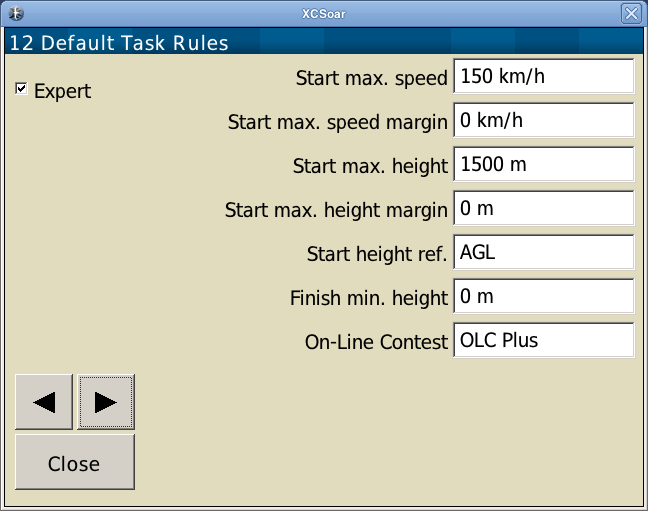
\includegraphics[angle=0,width=0.8\linewidth,keepaspectratio='true']{figures/config-rules.png}
\end{center}

\begin{description}
\item[Start max. speed*]  Maximum speed allowed in start observation zone.  Set 
  to 0 for no limit.
\item[Start max. speed margin*] Maximum speed above maximum start speed to tolerate. 
  Set to 0 for no tolerance.
\item[Start max. height*]  Maximum height above ground while starting the task. 
  Set to 0 for no limit.
\item[Start max. height margin*]  Maximum height above maximum start height to 
  tolerate.  Set to 0 for no tolerance.
\item[Start height ref.*]  Reference used for start max. height rule. \\
  {\bf MSL}: Reference is altitude above mean sea level. \\
  {\bf AGL}: Reference is the height above the start point.
\item[Finish min. height*]  Minimum height above ground while finishing the task. 
  Set to 0 for no limit. 
\item[OnLine Contest] Determines the rules used to optimize OnLine Contest 
  paths.  The implementation  conforms to the official release 2010, Sept. 23. \\
  {\bf OLC FAI}: Four points with common start and finish.  For tasks longer than
  500km, no leg less than 25\% or larger than 45\%; otherwise no leg less than 28\% 
  of total.  Finish height must not be lower than start height less 1000 meters. \\
  {\bf OLC Classic}: Up to seven points including start and finish, finish height
  must not be lower than start height less 1000 meters. \\
  {\bf OLC League}: A contest on top of the classic task optimisation, cutting
  a 2.5 hours segment over max. 3 of the turns. Finish height must not be below
  start height. \\
  {\bf OLC Plus}: A combination of Classic and FAI rules. 30\% of the FAI score
  are added to the Classic score. \\
  {\bf XContest}: tbd.
  {\bf DHV-XC}: tbd.
  {\bf SIS-AT}: tbd. 
\end{description}


%%%%%%%%%%%%%%%%%%
%\clearpage
\section{Default Task Turnpoint Types}

This page allows to set default turnpoint types used by the task editor. All 
options are well described for the task editor in chapter~\ref{cha:tasks}.


%%%%%%%%%%%%%%%%%%
\clearpage
\section{Devices} \label{conf:comdevices}

The Devices page is used to specify the ports used to communicate with
the GPS and other serial devices. The default settings are COM1 and
4800 bits per second.  When connected to the Vega intelligent
variometer, the settings should be COM1 and 38400.

\begin{center}
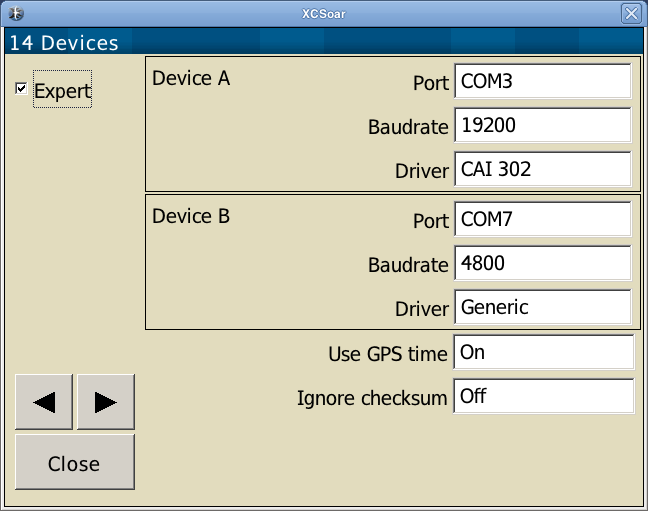
\includegraphics[angle=0,width=0.8\linewidth,keepaspectratio='true']{figures/config-devices.png}
\end{center}

Two COM devices are available (device A and device B), to allow, for
example, one to be connected to a GPS and another to be connected to a
second device such as a variometer.  If there is no second device, set
the device B port settings to the same as those of device A -- this
instructs the program to ignore device B.

The specific type of device can also be selected from a list in order
to enable support for devices with proprietary protocols or special
functions.

COM ports 0 to 10 may be used.  Which COM port is appropriate for you
depends on what make of PDA you use, and the communications medium
(serial cable, Bluetooth, virtual COM port, SD card or CF based GPS,
internal GPS).  Detailing the various options for different devices is
beyond the scope of this document.  If you have trouble identifying
which COM port to set, please refer to the XCSoar website and mailing
lists.

\begin{description}
\item[Use GPS time*] This option, if enabled sets the clock of the computer to 
  the GPS time once a fix is set. This is only necessary if your computer does 
  not have a real-time clock with battery backup or your computer 
  frequently runs out of battery power or otherwise loses time.
\item[Ignore checksum*] If your GPS device outputs invalid NMEA checksums, this 
  will allow it's data to be used anyway.
\end{description}


%%%%%%%%%%%%%%%%%%
\clearpage
\section{Logger}

This page allows you to set the pilot and aircraft details used for
annotating XCSoar's IGC logger. 

\begin{center}
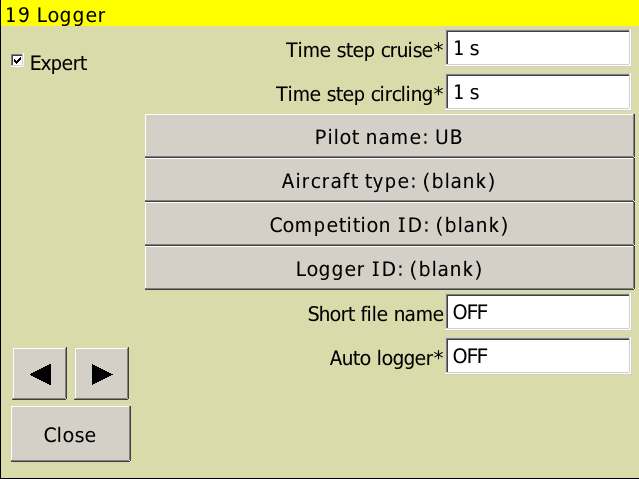
\includegraphics[angle=0,width=0.8\linewidth,keepaspectratio='true']{figures/config-logger.png}
\end{center}

\begin{description}
\item[Time step cruise*]  This is the time interval between logged points when 
  not circling. 
\item[Time step circling*]  This is the time interval between logged points when 
  circling. 
\item[Pilot name]  This is the pilot name used in the internal software logger 
  declaration.
\item[Aircraft type]  This is the aircraft type used in the internal software 
  logger declaration.
\item[Aircraft reg.]  This is the aircraft registration used in the internal 
  software logger declaration.
\item[Competition ID]  This is the aircraft competition ID.
\item[Logger ID]  This is the logger registration.
\item[Short file name*]  This determines whether the logger uses the short or the 
  long IGC file name.
\item[Auto logger*]  Enables the automatic starting and stopping of the logger
  on takeoff and landing respectively. Disable when flying paragliders to prevent 
  the low ground speeds from triggering the automatic logger.
\end{description}


%%%%%%%%%%%%%%%%%%
\clearpage
\section{Units}

This page allows you to set the units preferences used in all
displays, InfoBoxes, dialogues and input fields.  Separate selections
are available for speed, distance, lift rate, altitude, temperature, task
speed and latitude/longitude.

\begin{center}
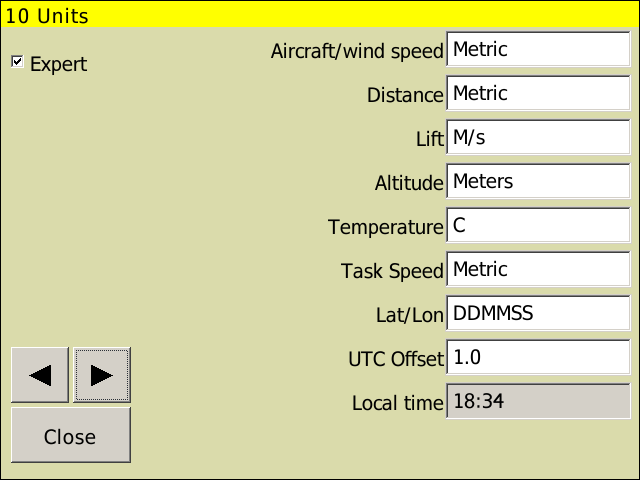
\includegraphics[angle=0,width=0.8\linewidth,keepaspectratio='true']{figures/config-units.png}
\end{center}

For most users hopefully one of the presets will match the needs.  The presets 
include unit sets for {\bf American}, {\bf Australian}, {\bf British}, 
and {\bf European}.

The UTC offset field allows the UTC local time offset to be specified.
The local time is displayed below in order to make it easier to verify
the correct offset has been entered.  Offsets to the half-hour may be
set.


%%%%%%%%%%%%%%%%%%
\clearpage
\section{User Interface}\label{sec:interface}

This page allows to customise the way the user controls and interacts with
XCSoar.

\begin{center}
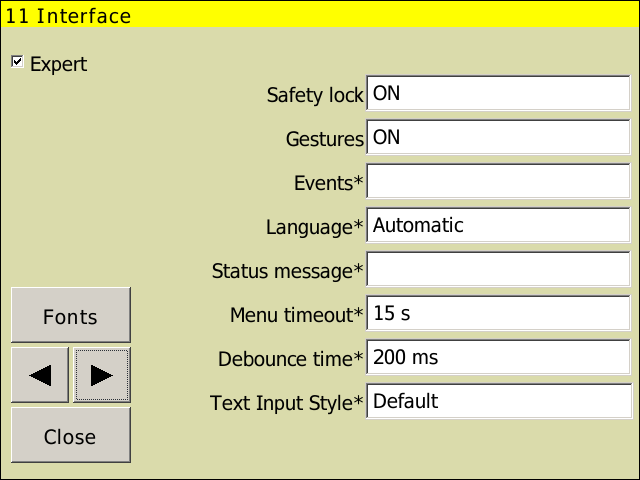
\includegraphics[angle=0,width=0.8\linewidth,keepaspectratio='true']{figures/config-interface.png}
\end{center}

\begin{description}
\item[Auto Blank*] This determines whether to blank the display after a long
  period of inactivity when operating on internal battery power (visible for PDA
  only).
\item[Events*]  The Input Events file defines the menu system and how XCSoar
  responds to button presses and events from external devices.
\item[Language]  The language options selects translations for English texts to
  other languages.  Select {\bf English} for a native interface, {\bf Automatic}
  to localise XCSoar according to the system settings; or you may select one of 
  the two character language short cuts directly.
\item[Status message*]  The status message file can be used to define sounds to 
  be played when certain events occur, and how long various status messages will 
  appear on screen.
\item[Menu timeout*]  This determines how long menus will appear on screen if the user
  does not make any button presses or interacts with the computer.
\item[Debounce timeout*]  This is the minimum interval between the system 
  recognising key presses.  Set this to a low value for a more responsive user 
  interface; if it is too low, then accidental multiple key presses can occur.
\item[Text Input Style*]  Determines which style for text entries is used. 
  See Section~\ref{sec:textentry} for further information on textual input. \\
  {\bf HighScore Style}: For entering text you have to change the underlined 
  character to the relevant letter. \\
  {\bf Keyboard}: Uses the on-screen keyboard for entering text. \\
  {\bf Default}: Uses the default input style for your platform.
\end{description}

Some Pocket PC devices have poorly designed keys that are subject to
accidental multiple key presses, which is known as key `bouncing'.  The
de-bounce timeout sets a minimum time between successive key presses
that is detected by XCSoar, to alleviate this problem.  If this value
is set very high, then the user interface will feel unresponsive; if
the value is set too low, then bouncing may occur.

Press the \button{Fonts} button to adjust the fonts XCSoar uses.


%%%%%%%%%%%%%%%%%%
\clearpage
\section{Fonts}

This page enables customization of fonts in various fields of the program.

\begin{center}
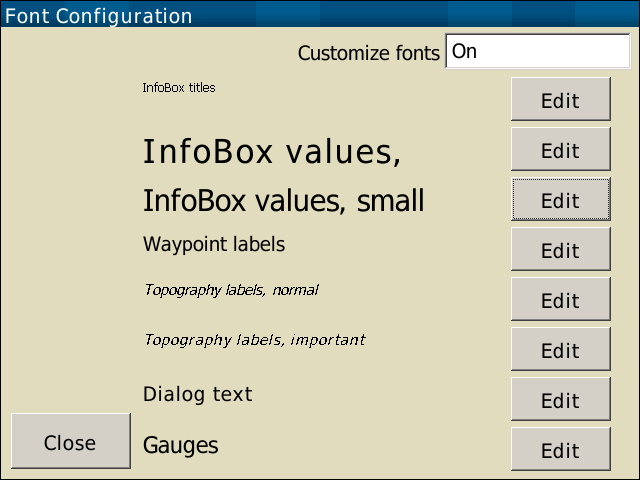
\includegraphics[angle=0,width=0.8\linewidth,keepaspectratio='true']{figures/config-fonts.png}
\end{center}

Once the customization is enabled, the \button{Edit} buttons allow to change some parameters (Font 
Face, Height, Bold and Italic) of the chosen font.

If customization is disabled, default fonts will be used.

%%%%%%%%%%%%%%%%%%
\clearpage
\section{Symbols}\label{sec:symbols}

This page provides options relating to the items overlaying the map display.

\begin{center}
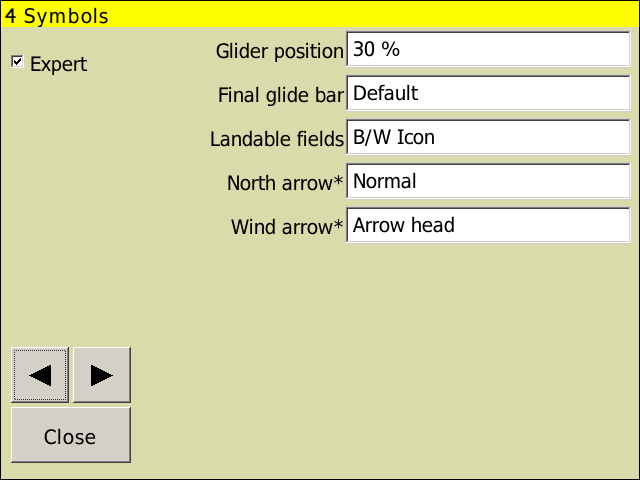
\includegraphics[angle=0,width=0.8\linewidth,keepaspectratio='true']{figures/config-symbols.png}
\end{center}

\begin{description}


\item[Final glide bar]  Two styles are available: Default and
Alternate. The differences between these styles is cosmetic.  Alternate displays the height difference to the 
right of the final glide bar; default displays the height difference above/below the final glide bar and inside a 
rounded box.

\item[North arrow*]  Two styles are available.  Normal, or with a white outline.
\end{description}






%%%%%%%%%%
\clearpage
\section{Layout}

This page defines various display styles used by symbols and InfoBoxes.

\begin{center}
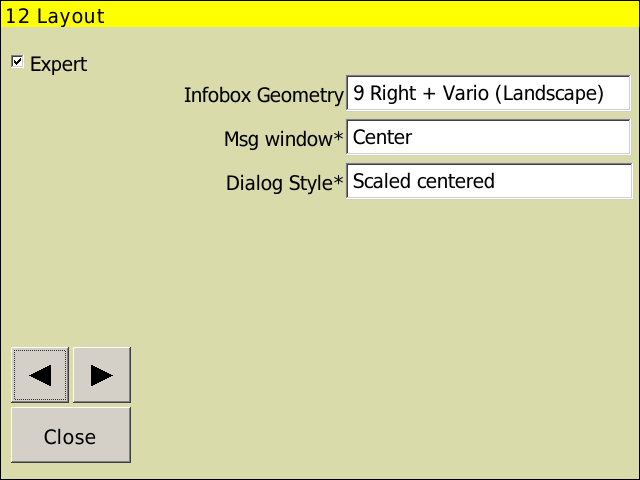
\includegraphics[angle=0,width=0.8\linewidth,keepaspectratio='true']{figures/config-layout.png}
\end{center}

\begin{description}
\item[Infobox Geometry]  Sets the geometry values for InfoBoxes. In landscape
mode InfoBoxes are placed left and right, in portrait mode top and bottom of the screen. The numbers in front refer 
to the total number of InfoBoxes.
\item[Msg window*]  Defines the alignment of the status message box, either
centred or in the top left corner.
\item[Dialogue style*]  Determines the display size of dialogues.
\end{description}




%%%%%%%%%%

\clearpage
\section{{\InfoBox}es}

This page allows the configuration of four InfoBox sets to be defined for each
display mode (circling, cruise, final glide) and one auxiliary set.  See
Section~\ref{cha:infobox} for a description of the InfoBox types and their meanings.

\begin{center}
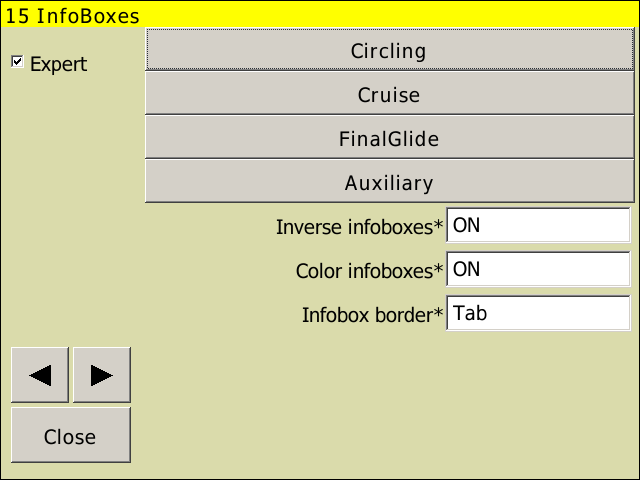
\includegraphics[angle=0,width=0.8\linewidth,keepaspectratio='true']{figures/config-infoboxes.png}
\end{center}

To arrange a set of InfoBoxes press one of the buttons labeled with the name
of the set.  The InfoBoxes are numbered; the location of the InfoBoxes depends
on the screen geometry.  The table below shows the InfoBox numbers for landscape screen layout (Altair):

\begin{tabular}{|c|c|}
\hline
1 &  \\
\hline
2 &  \\
\hline
3 &  \\
\hline
4 & 7 \\
\hline
5 & 8 \\
\hline
6 & 9 \\
\hline
\end{tabular}

The table below shows the InfoBox numbering for portrait screen layout:

\begin{tabular}{|c|c|c|c|}
\hline
1 & 2 & 3 & 4 \\
\hline
\hline
5 & 6 & 7 & 8 \\
\hline
\end{tabular}

\begin{description}
\item[Inverse InfoBoxes*]  If true, the InfoBoxes are white on black, otherwise black on white.
\item[Colour InfoBoxes*]  If true, certain InfoBoxes will have coloured text. For example, the 
active waypoint InfoBox will be blue when the glider is above final glide.
\item[Infobox border*]  Two styles for InfoBox borders are available: `Box'
draws boxes around each InfoBox.  `Tab' draws a tab at the top of the InfoBox across the title.
\end{description}



%%%%%%%%%%

\clearpage
\section{Experimental features}

This page provides experimental features which are not finished yet.

\begin{center}
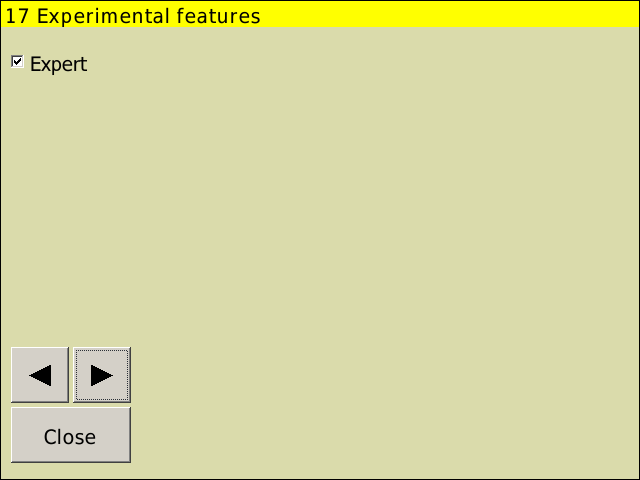
\includegraphics[angle=0,width=0.8\linewidth,keepaspectratio='true']{figures/config-exp.png}
\end{center}

\begin{description}
\item[Device model] This setting allows the adaptation to specific hardware
XCSoar runs on (visible for PDA only).
\end{description}
